%% ma: L12-B01-0035
%% lop: 12
%% chuong: 1
%% bai: 1
%% dang: 12.1.11
%% loai: TN4
%% muc: NB
%% dap_an: "B"
%% nguon: "HK1-DeOn_1_1.pdf (M10, Đề ôn tập học kì 1 Toán 12, Đề số 2), Phần I Câu 4"
%% kien_thuc: "Bài 1 (tính đơn điệu và cực trị)"
%% trang_thai: chinh-thuc
%% ghi_chu: "Đọc điểm cực tiểu (dạng 12.1.11 là đọc điểm cực đại từ bảng biến thiên; cùng mô hình và cùng thao tác)."
\begin{ex}
Cho hàm số $y=f(x)$ có bảng biến thiên như sau:
\begin{center}\begin{tikzpicture}
\tkzTabInit[lgt=1.2,espcl=2.4]{$x$/.8,$y'$/.8,$y$/2.2}{$-\infty$,$-1$,$2$,$+\infty$}
\tkzTabLine{,+,0,-,0,+,}
\tkzTabVar{-/$-\infty$,+/$1$,-/$-2$,+/$+\infty$}
\end{tikzpicture}\end{center}
Hàm số đã cho đạt cực tiểu tại
\choice{$x=-2$}{\True $x=2$}{$x=1$}{$x=-1$}
\loigiai{$f'(x)$ đổi dấu từ âm sang dương khi đi qua $x=2$ nên hàm số đạt cực tiểu tại $x=2$.}
\end{ex}
